\chapter{Monads}
\section{Overview}
\subsection{Side effect}
In imperative language like C/C++ , it is often the case that it access the variable outside the function,eg. the error flag.In Java, the keyword \textbf{synchronized} is used to acquire look to the share resource,most of time,they are the resource from out side word.Imperative language are unrestricted to side effect,which makes it hard to write function that allows parallelism .On the other hand,Haskell restricts side effects with a static type system; it uses the concept of monads to do stateful and IO computations.[Imperative Functional Programming]

\subsection{Monad}
sions.
Another approach to introducing effects in a purely functional language
is to make the use of effects explicit in the type system. Several methods
have been proposed, but the most elegant and widely used is the concept
of a monad.[Imperative Functional Programming]  Monads in Haskel have been used to model IO,state,logger,error as well as List.




\section{Haskell and Category Theory}
Category theory is a general theory that examine and organize mathematical object like set ,function,function domains Cartesian-set.

A Category $C $ in category theory is defined below :
\begin{enumerate}
\item a collection of objects 
\item a collection of arrows (often call morphism) 
\item operations assigning to each arrow $f$ an object $dom\;f$,its domain ,and an object $cod\;f$,its co domain.
\item a composition operator assigning to each pair of arrows $f and g$,with $cod\;f = dom\;g$,a composite arrow $ g \circ f:dom\;f \rightarrow  cod\;g$ , satisfying the following associative law: \\
For any arrow $f: A \rightarrow B,g:B \rightarrow C,and\;h: C\rightarrow D$(with A,B,C and D not necessarily distinct),
$$h\circ (g\circ f) = (h\circ g)\circ f$$
\item for each object A, an identify arrow $id_{a}: A \rightarrow A$ satisfying the following identity law:\\
For any arrow $ f: A \rightarrow B,$ 
$$ id_{a} \circ f = f  \;and\;  f\circ id_{a} = f. $$
\end{enumerate}\cite{pierce_basic_1991}


\subsubsection*{Category in Haskell}
In Haskell,all the type in can be view as objects and all the function can be view as arrows.id function has been defined as follow.
\begin{hcode}
 id :: a -> a
\end{hcode}
It can be viewed as an identify arrow of all objects(types).
\subsubsection*{Functor in Haskell}
Some high order function like fmap can be view as a functor.
\begin{hcode}
fmap :: (a -> b) -> (f a -> f b)
\end{hcode}
From its signature we know that fmap maps arrows in category to another category.f a is the type constructor that takes a as its parameter an generate f a as a new type.So it maps the arrow from a $->$ b to f a $->$ f b.

Its instances types like Maybe and ReadP satisfy the functor law:
\begin{hcode}
fmap id  ==  id
fmap (f . g)  ==  fmap f . fmap g
\end{hcode}

Functions are the first member of the program in functional programming,since no size affect is not allow ,there should be a way to combine the all kinds of functions to from a new function instead of just simply chain the input output of each function as the former will generate intermediate output.


For instance ,counting the file of java source code in current directory can be written as follow:


	$$ ls-al . | grep *.txt| wc -l $$ 
	
	
To substantiate the this concept , let's use the map/fold fusion technique of Haskell as an example.

If we want to calculate the sum of the square of each element of a list eg. [1,3,4,6,7,9],the result of it is  $ 1^2+3^2+4^2+6^2+7^2+9^2=192 $.In Haskell ,we could use map and fold to address problem.

 %list_of_square = map (^2)
%sum_of_list = foldr (+) 0
%sum_of_square =   sum_of_list.list_of_square

To avoid generating intermediate output from the first function to second function, the could rewite the hold function using a single fold

The all map/fusion is is equivalent to 
$ foldr f e . map g = foldr (\\x y -> f (g x) y) e $

therefore, the 

$ sum_of_square = foldr (\\x y -> x^2 + y) 0 $





\section{Monadic Function}
\subsection{Data Type Constructor}
Type constructors play a fundamental role in Haskell's monad support.
\subsection{Monadic Function}
A monadic function is function that produce , however,monadic function like \textbf{putStr :: String -$>$ IO ()} can not be combined using \\ \textbf{(.) :: (b -$>$ c) -$>$ (a -$>$ b) -$>$ a -$>$ c}.Monadic class constructor has tag 



\section{Monads}
In Haskell,monad is used an abstract data type constructor to represent multiple kinds of computation such as a computation that will do IO action,or a computation that has state.Those computations are in-pure because that manipulate the outside world.In Haskell.Mathematically, monads are governed by set of laws that should hold for the monadic operations [A Gentle Introduction to Haskell, Version 98]. There are two basic law in monads ,they are bind return .The Monad class is defined as follow:
\begin{hcode}
class Monad m where
  (>>=) :: m a -> (a -> m b) -> m b
  (>>) :: m a -> m b -> m b
  return :: a -> m a
  fail :: String -> m a
\end{hcode}

The return function can inject a value into monadic type.
The bind function can combine two monadic function, one should be of type \textbf{m a} and another should be of type \textbf{a -$>$ m b} .

Beside this two function,Haskell also provide other monadic operator which all derive from \textbf{return} and \textbf{bind},they are:
\begin{hexample}
liftM :: (Monad m) => (a1 -> r) -> m a1 -> m r
liftM2  :: (Monad m) => (a1 -> a2 -> r) -> m a1 -> m a2 -> m r
ap :: (Monad m) => m (a -> b) -> m a -> m b
(=<<) :: (Monad m) => (a -> m b) -> m a -> m b
\$ ::(m a -> m b) -> m a -> m b 
\end{hexample}

These monadic operation is define using the bind and return.For example ,liftM is defined by bind and return like 
\begin{hcode}
liftM f m1              = do { x1 <- m1; return (f x1) }
\end{hcode}
Therefore,when defining a monad,only bind and return need to be specified.

\subsubsection{Monadic Characteristic}
For all monad instance ,beside define three monadic operator ,they must apply three compulsory monad laws:

\begin{hcode}
"Left identity": return a >>= f  ≡  f a
"Right identity": m >>= return  ≡  m
"Associativity": (m >>= f) >>= g  ≡  m >>= (\x -> f x >>= g)
\end{hcode}

In monad instance ,these monad laws will become a restriction of the operation when combining monadic function using monadic operation,these restriction will be discussed in following sections.


\subsection{IO Monad}
Haskell use IO monad to limit the IO sequence.Monadic operation are used to represent IO processing pipeline.\\

Haskell I/O has always been a source of confusion and surprises for new Haskellers.

Normally, the first thing to lean a new language to to print something on the screen,but it is not the case in Haskell.The first thing I do in Haskell is to write a quick sort algorithm which is a classic program to show the powerful Haskell list comprehension feature that brings the most elegant solution of quick sort compared to most of other language.On the other hand,its not that straight forward to build an IO system upon it inside language that emphasized purity.



It probably not the best monad for beginner to learn as it dost not provide escape function.The IO moand is implemented as part of language in \textbf{Base.GHC},thus the logic of monad operator is not exposed to outside world.

\begin{hcode}
unsafePerformIO :: IO a -> a
\end{hcode}

The above shows the code of an escape function which will break the purity of Haskell IO system.This is the "back door" into the IO monad, allowing IO computation to be performed at any time. For this to be safe, the IO computation should be free of side effects and independent of its environment.[ haskell io document]


As we can guess from the nature of Haskell,IO monad is introduced to guarantee to following factor,

\begin{itemize}
\item The sequence of IO actions perform in a lazy Haskell context.
\item perform IO as an function rather than a function or and command in functional programming context.
\item combine IO,distinguish computation that with IO actions with the one without.
\item  file buffering , open and close file in a correct manner.
\end{itemize}


The code below shows combination of monad using bind operator.
\begin{hcode}
ioAction 
  =putStrLn "What is your name ?"
	 >>= (_-> getLine >>= 
		(\x -> putStrLn ("welcome" ++ x) ))
\end{hcode}



\subsection{State Monad}
The basic idea of a state monad is to allow us to represent functions which interact with local state variables (which are just called local variables in most languages), or global state variables (usually called global variables). Essentially, they allow us to simulate some aspects of imperative programming in a purely functional setting.\\

An alternate solution is that we can pass the initial state into each function and return the state together with the result,with may looks like,
\begin{hcode}
add :: State -> Input -> (State ,Output)
-- implement

subtract :: State -> Input -> (State,Output)
\end{hcode}


To make it possible to composite computation with state we could rewrite all computation with follow.

\begin{hcode}
add :: (Input,State) -> (Output,State)
-- implementation 
subtract :: (Input,State) -> (Output,State)
combine = add.subtract 
\end{hcode}

However,its tedious to write all the function with computation this way.The state monad provides a way to encapsulate the state logic into a monad without explicitly specify a State type as input and output.Like IO, the computations with state  are tagged with the type constructor \textbf{State} indicating this is a state monadic function.Most importantly, the monad law and state monad implementation guarantee the follow fact of a computation with state , they are

\begin{itemize}
\item It possible to construct a new state monadic function without initial state.
\item when combine two state,from the nature of state transformation ,the change of state of  the second function is always after the first function.
\item For a computation with state,we need to need the both the result of computation as well as the final state as an output of the computation.
\end{itemize}

\begin{figure}[H]
  \centering
	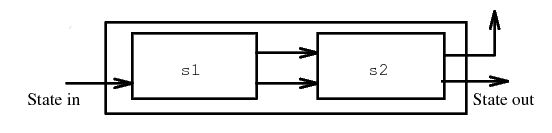
\includegraphics[width=0.80\textwidth]{pic/c3/state_monad.png}
	\caption{Combining Two "Stateful" Monadic Functions}
\end{figure}


\subsection{List Comprehension and List Monad}
\subsection{List Comprehension}
Haskell added syntax sugar to allow programmer to write code in a more readable manner.The list comprehension allow us to write a list using mathematics favour.

A Fibonacci series can be written as follow,
\begin{hcode}
fibs :: [Int]
fibs = 0 :1 : [ a + b | (a, b) <- zip fibs (tail fibs)]
\end{hcode}

If we view if as a mathematical expression,we can easily figure out it means $ \lbrace  0,1 ,(0+1),(1+1),(1+2),(2+3),(3+5),... \rbrace $, which will generate a Fibonacci series.In addition,it is also an example of how useful of lazy evaluation is in Haskell.

\subsection{List Monad}
We can view a list as monad.In list comprehension ,we have the \textbf{$<$-} operator which we can view it as $\in$,which has a mathematical $ in$  semantic.\\

Alternatively , 
\section{Using Monad Operator to Combine Monadic Function}

\section{Type system in Haskell}
\section{Do Notation }
The do notation is a syntax sugar to write monadic operation especially bind in a imperative way ,to be more specified,only monadic function with the same return type can write together.An IO action that return \textbf{IO ()} can not put with and state monadic function that return \textbf{State s a}.

To write a get line and put line logic using bind, the sequence of IO is guaranteed by monad laws.
\begin{hcode}
 getLine >>= (\x -> putStrLn x)
\end{hcode}


Following code shows that the same functionalities are written using do-notation,which shows a strong similarity to a imperative language.
\begin{hcode}
do line <- getLine 
   putStrLn line
\end{hcode}


